
\label{sec:non_disspers_KDO_section}
На рис. \ref{ris:non_disspers_kdo} приведены бездисперсионные двухкристальные КДО, рассчитанные в соответсвии
с выражением (\ref{eq:doudle_spectra_angle_map_on_detector}). В качестве кристалла-монохроматора
и образца был выбран монокристалл кремния с системой отражающих плоскостей (220), эксперимент проводился в
соответсвии со схемой, представленной на рис. \ref{ris:double_crystal_schem_lamtet_a}.

\begin{figure}[H]
  \centering
  \subfloat[]{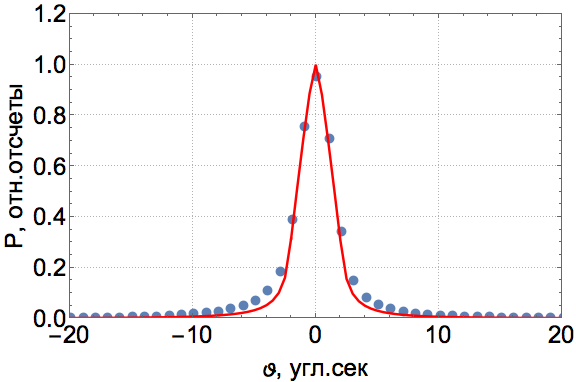
\includegraphics[width=0.45\textwidth]{images/non_disspers_20_40.png}\label{fig:f1}}
  \hfill
  \subfloat[]{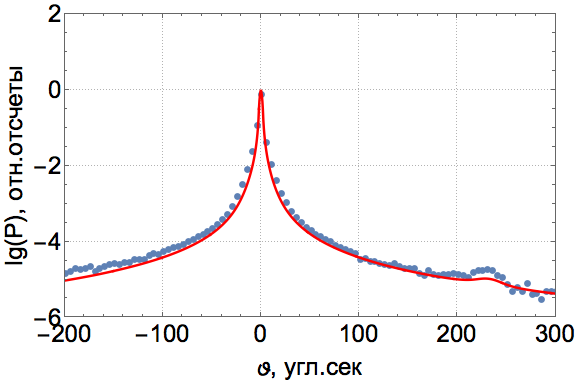
\includegraphics[width=0.45\textwidth]{images/non_disspers_20_40_log.png}\label{fig:non_disspers_kdo_1}}
  \hfill
  \subfloat[]{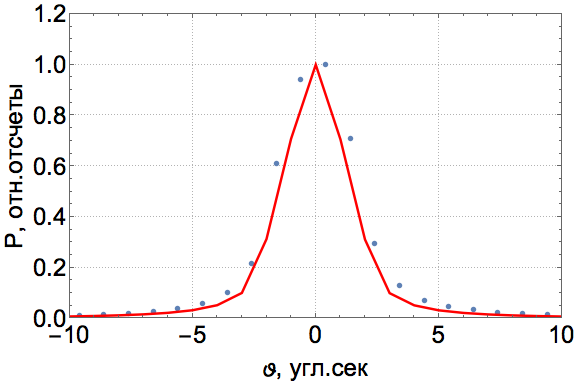
\includegraphics[width=0.45\textwidth]{images/non_disspers_300_200.png}\label{fig:f2}}
  \hfill
  \subfloat[]{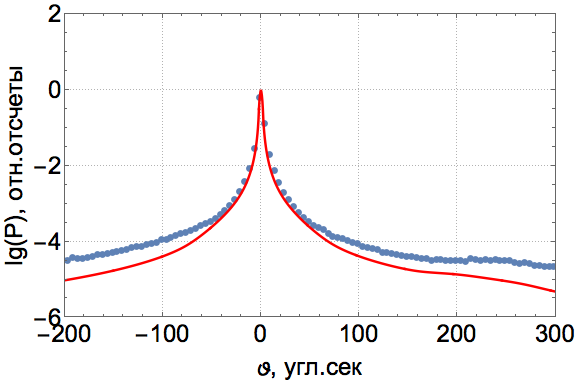
\includegraphics[width=0.45\textwidth]{images/non_disspers_300_200_log.png}\label{fig:f2}}
  \caption{Двухкристальная бездисперсионная КДО $MoK_{\alpha}$ - излучения для схемы с установленными
   кристаллом-монохроматором Si(220) и образцом Si(220). Расстояние до щелевых коллиматоров
  составляет $L_1= 570 $мм, $L_2 = 1005$ мм соответсвенно.
  Линейный размер источника $\delta = 0.1$ мм. Расчет - (красная линия), эксперимент - (синие точки).
  Результаты приведены для размеров щелевых коллиматоров  $S_1 = 20 $ мкм; $ S_2 = 40$ мкм (a),
    $S_1 = 20 $ мкм; $ S_2 = 40$ мкм (b),
   $S_1 = 300 $ мкм; $ S_2 = 200$ мкм (c),
    $S_1 = 300 $ мкм; $ S_2 = 200$ мкм (d)}
  \label{ris:non_disspers_kdo}
\end{figure}

На рис. \ref{fig:non_disspers_kdo_1} видно, что наряду с главным пиком, соответствующим $K_{\alpha1}$ - линии
излучения, на которую настроен монохроматор, присутствует вклад от соседней характеристической линии
 $K_{\alpha2}$. Впервые, на это свойство двухкристальных КДО, получаемых в бездисперсионной
схеме в случае использования рентгеновской трубки было указано авторами работы \cite{chuev2008}.

\begin{figure}[H]
  \centering
  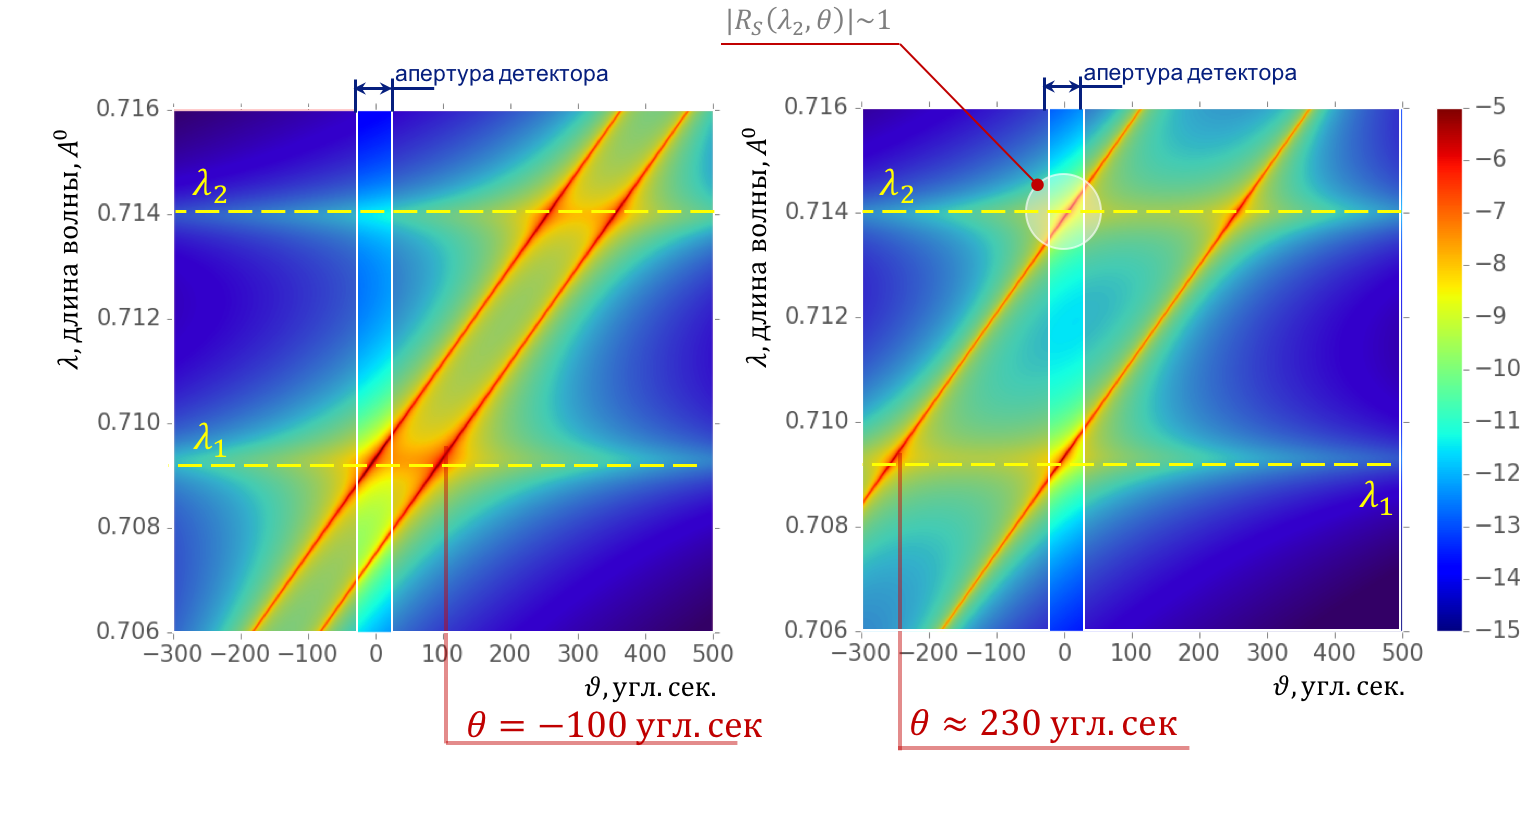
\includegraphics[width=0.8\textwidth]{images/vklad_kalpha2.png}
  \caption{Схематичное объяснение эффекта образования дополнительного пика на двухкристальных КДО
  с помощью спектрально-углового представления}
  \label{ris:vklad_kalpha2}
\end{figure}

На рис. \ref{ris:vklad_kalpha2} наглядно изображен механизм формирования дополнительного пика,
соответствующего $K_{\alpha 2}$ - составляющей спектра. В точке образования пика ($\theta = 230$ угл.сек.), коэффициент
отражения  (см. \ref{eq:doudle_spectra_angle_map_on_detector})
для кристалла образца при длине волны $\lambda_2$ максимален (в случае кристалла Si равен 1). Но отражение
от монохроматора в этой точке является слабым, т.о. интенсивность дополнительного пика на 5 порядков меньше
интенсивности основного, в отличие от того случая, когда реализуется сильное отражение от обоих кристаллов.
 Необходимо отметить, что пик физически существует вне зависимости от размера щелевых коллиматоров, но
при достаточно больших размерах щелей (200 мкм.) пропадает на фоне хвостов КДО $K{\alpha 1}$ - линии.
